\textbf{A few words on epigenomic data}

We illustrate the performances of DEScan2 using a dataset \cite{Su2017} that describes in vivo adult mouse dentate granule neurons before and after synchronous neuronal activation using Atac-Seq and RNA-Seq technologies (see sections \ref{sec:atacseq} and \ref{sec:rnaseq} for a description of these sequencing techniques).

This dataset is organized in 62 samples of Atac-Seq and RNA-Seq, extracted at different time points, with four replicates at each time point.
We chose to compare the differences at the first two stages, time 0 (E0) and 1 hour after neuronal induction (E1), in order to show a possible Atac-Sec workflow for Differential Enrichment, and how to integrate this data type with RNA-Seq. A general illustration of our dataset is represented in \ref{fig:atacdataset}.

\begin{figure}[H]
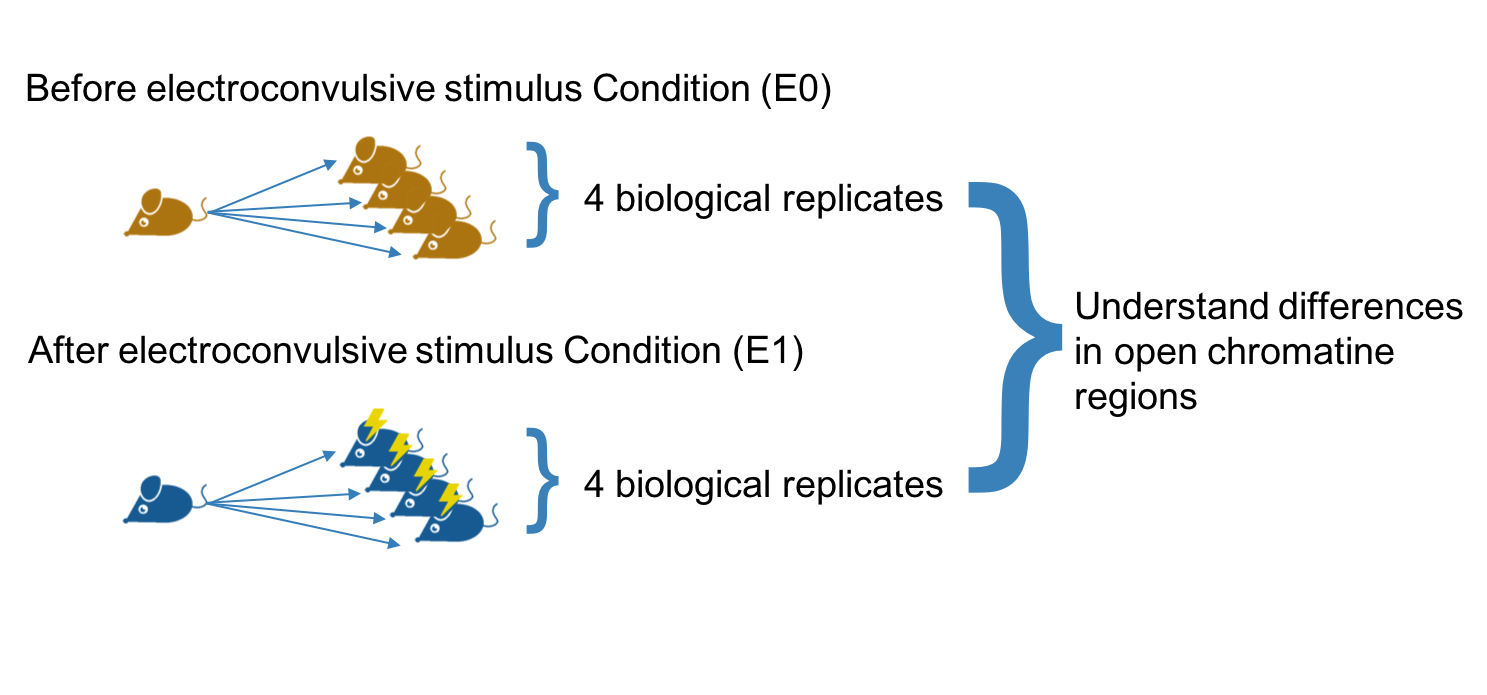
\includegraphics[width=\textwidth,height=\textheight,keepaspectratio]{img/descan2/dataset.png}
\caption[DEScan2 dataset illustration]{An illustration of our extraction of the \cite{Su2017} dataset.}
\label{fig:atacdataset}
\centering
\end{figure}

We downloaded the data from \textit{GEO} database \cite{Edgar2002, Barrett2013} with accession number GSE82015\footnote{\url{https://www.ncbi.nlm.nih.gov/geo/query/acc.cgi?acc=GSE82015}} and mapped raw data using \textit{STAR} \cite{Dobin2013} with default parameter on Mus Musculus Genome ver.10 (mm10).

In order to detect the open chromatin regions we run our peak caller, cutting the genome in bins of 50bp and using running windows of minimum 50bp and maximum 1000bp. In such a way we are able to detect not just broad peak, but also smaller peaks.

To be confident with our results we compared the DEScan2 detected peaks with the same validated regions (Arc and Gabrr1) in the original work \cite{Su2017}.
The lower part of figure \ref{fig:peaksdescan} shows the detected and validated regions (in blue and red) resulting differentially enriched between the E0 (in pink) and E1 (in green) conditions, while the upper part shows DEScan2 peaks (in blue), highlighting a capability to catch not only the same regions of the published ones, but also (gold circles) to be more careful in the smaller peaks detection.

\begin{figure}[H]
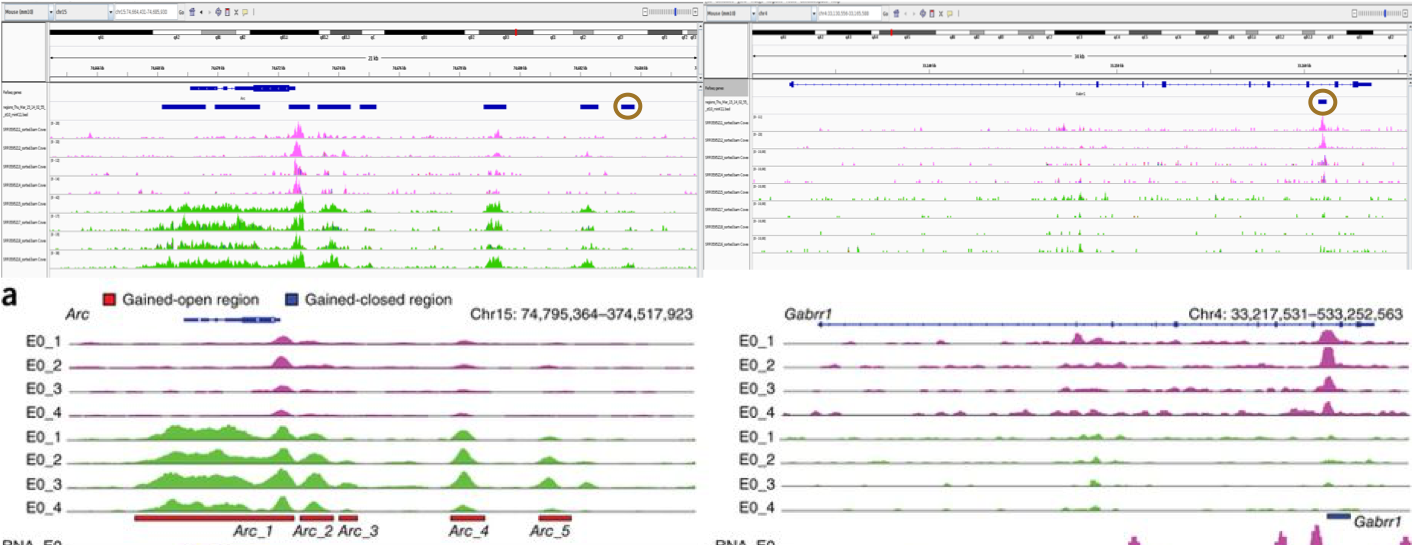
\includegraphics[width=\textwidth,height=\textheight,keepaspectratio]{img/descan2/peaks.png}
\caption[DEScan2 peaks detection]{A comparison of DEScan2 detected peaks with validated peaks in article \cite{Su2017}.}
\label{fig:peaksdescan}
\centering
\end{figure}

While it is very important to detect good peaks with a peak caller, it seems to be more relevant to detect reliable regions. Indeed, during the filtering step, the number of peaks depends not only by the peak score, but also by the number of replicates designed in the experiment.
The figure \ref{fig:filteringdescan} puts in relation these two relevant information. 
On the x-axis is represented the number of replicates, while on the y-axis is traced the number of peaks, and each curve represents a different threshold on the peaks score, showing that higher are the thresholds on the scores and the number of replicates, lower is the number of the detected peaks.
Highlighting a proportional inversion between the number of the peaks and the combination of the number of samples and the detected regions score.


\begin{figure}[H]
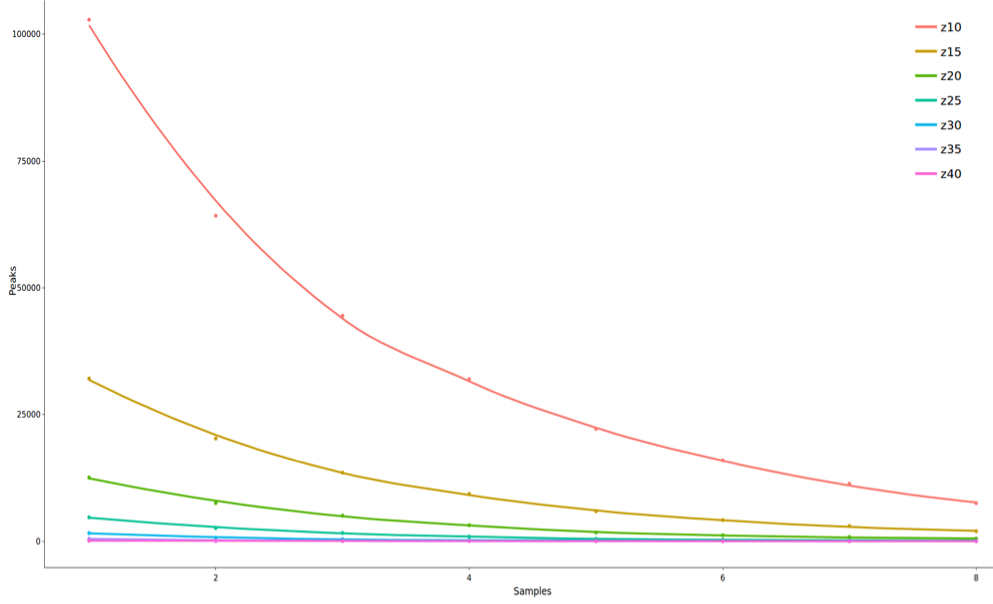
\includegraphics[width=\textwidth, height=\textheight, keepaspectratio]{img/descan2/filtering.png}
\caption[DEScan2 filtering step]{Filtering the detected regions with different thresholds on peak scores.}
\label{fig:filteringdescan}
\centering
\end{figure}

The filtered-in regions can be processed by DEScan2 in order to obtain a count matrix with samples on the columns and peaks on the rows.
This type of data structure is very versatile, because it enables to perform several operations, like the differential enrichment of regions (DERs) and, if possible, the integration with other kind of omics, as RNA-Seq.

In order to preserve the information associated to the peaks, DEScan2 produces as output a \textit{SummarizedExperiment} (figure \ref{fig:countsdescan}) data structure, which enables to retrieve the count matrix with \lstinline{assays} method, and to access the peaks information in \textit{GenomicRanges} format with the \lstinline{rowRanges} method.

\begin{figure}[H]
\centering
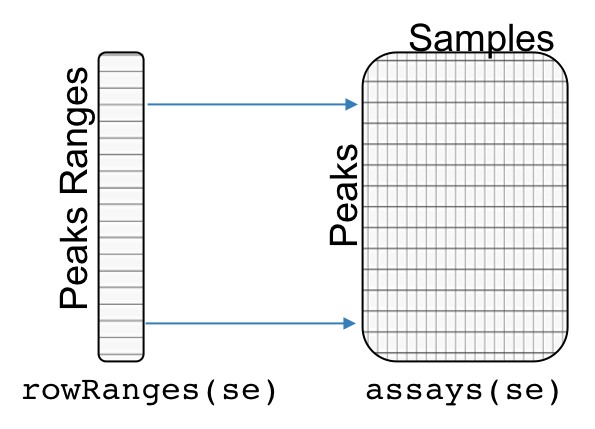
\includegraphics[keepaspectratio]{img/descan2/counts.png}
\caption[DEScan2 counts illustration]{An illustration of the \textit{SummarizedExperiment} data structure produced by DEScan2.}
\label{fig:countsdescan}
\centering
\end{figure}

Before to proceed to detect DERs, it is a good standard to normalize the data, also because without any kind of normalization we are not able to detect any DERs.
The nature of the data, in count format, makes it possible to apply several well known RNA-Seq normalizations techniques, as \textit{TMM}, \textit{upper-quartile}, \textit{full-quantile}, \textit{RUV-Seq}, etc \cite{Risso2014, Robinson2010, Dillies2013}.

While the \textit{TMM} and \textit{upper-quartile} normalizations modify the data in a way that makes it impossible to detect DERs, other kind of normalizations and combinantions of them give good results.

The figure \ref{fig:normalizationsdescan} sintetizes this concept very well, highlighting a relation between the number of DERs and the minumum number of samples used for filtering the data during the DEScan2 filtering step.

The plot shows that \textit{upper-quantile}, even if combined with \textit{RUV-Seq} normalization, is not able to linearly detect a good amount of DERs, while \textit{full-quantile}, when combined with \textit{RUV-Seq} seems to affect the data in a way that overdetect the number of DERs. 
When looking at the \textit{full-quantile} and \textit{RUV-Seq} by themself seem to perform better than the other normalizations. The first one has a downhill almost linear, while the second one has a very fast downhill with a regrowth when the number of samples is higher.

Even if these normalization methods show good performances with this type of epignomic data, our investigations suggest that for sure more testing is required, but maybe an ad-hoc normalization method for these data has to be developed.

\begin{figure}[H]
\centering
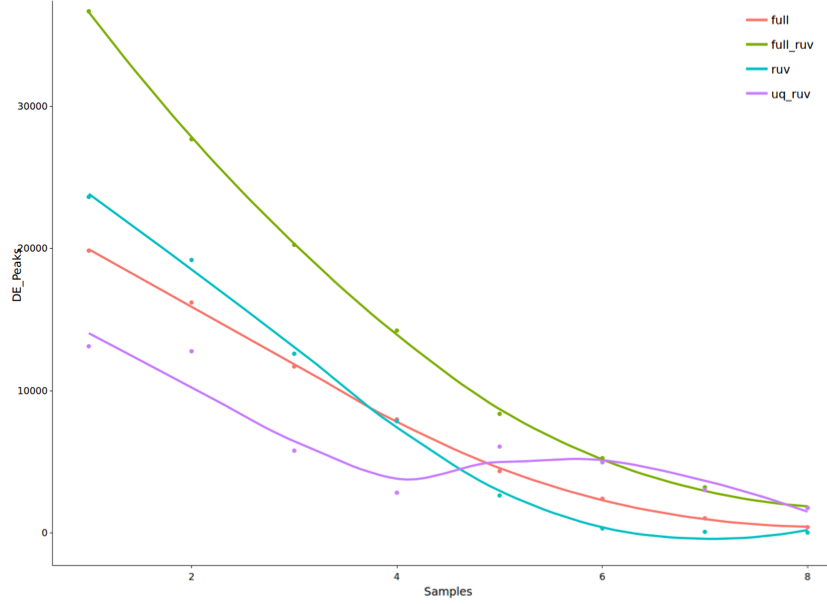
\includegraphics[width=\textwidth, height=\textheight, keepaspectratio]{img/descan2/normalizations.png}
\caption[Normalizations applied to detected regions]{The figure shows the effects of different normalizations on the epigenomic differentially enriched regions.}
\label{fig:normalizationsdescan}
\centering
\end{figure}

To estimate the DERs any of the RNA-Seq methods can be applied, such as \textit{DESeq2}, \textit{edgeR}, \textit{NOISeq}, etc \cite{Robinson2009, McCarthy2012, Tarazona2012}.

In this case, we decided to use \textit{edgeR} package, because of its usage flexibility and the possibility to better tune the design of the experiment.

\begin{figure}[H]
\centering
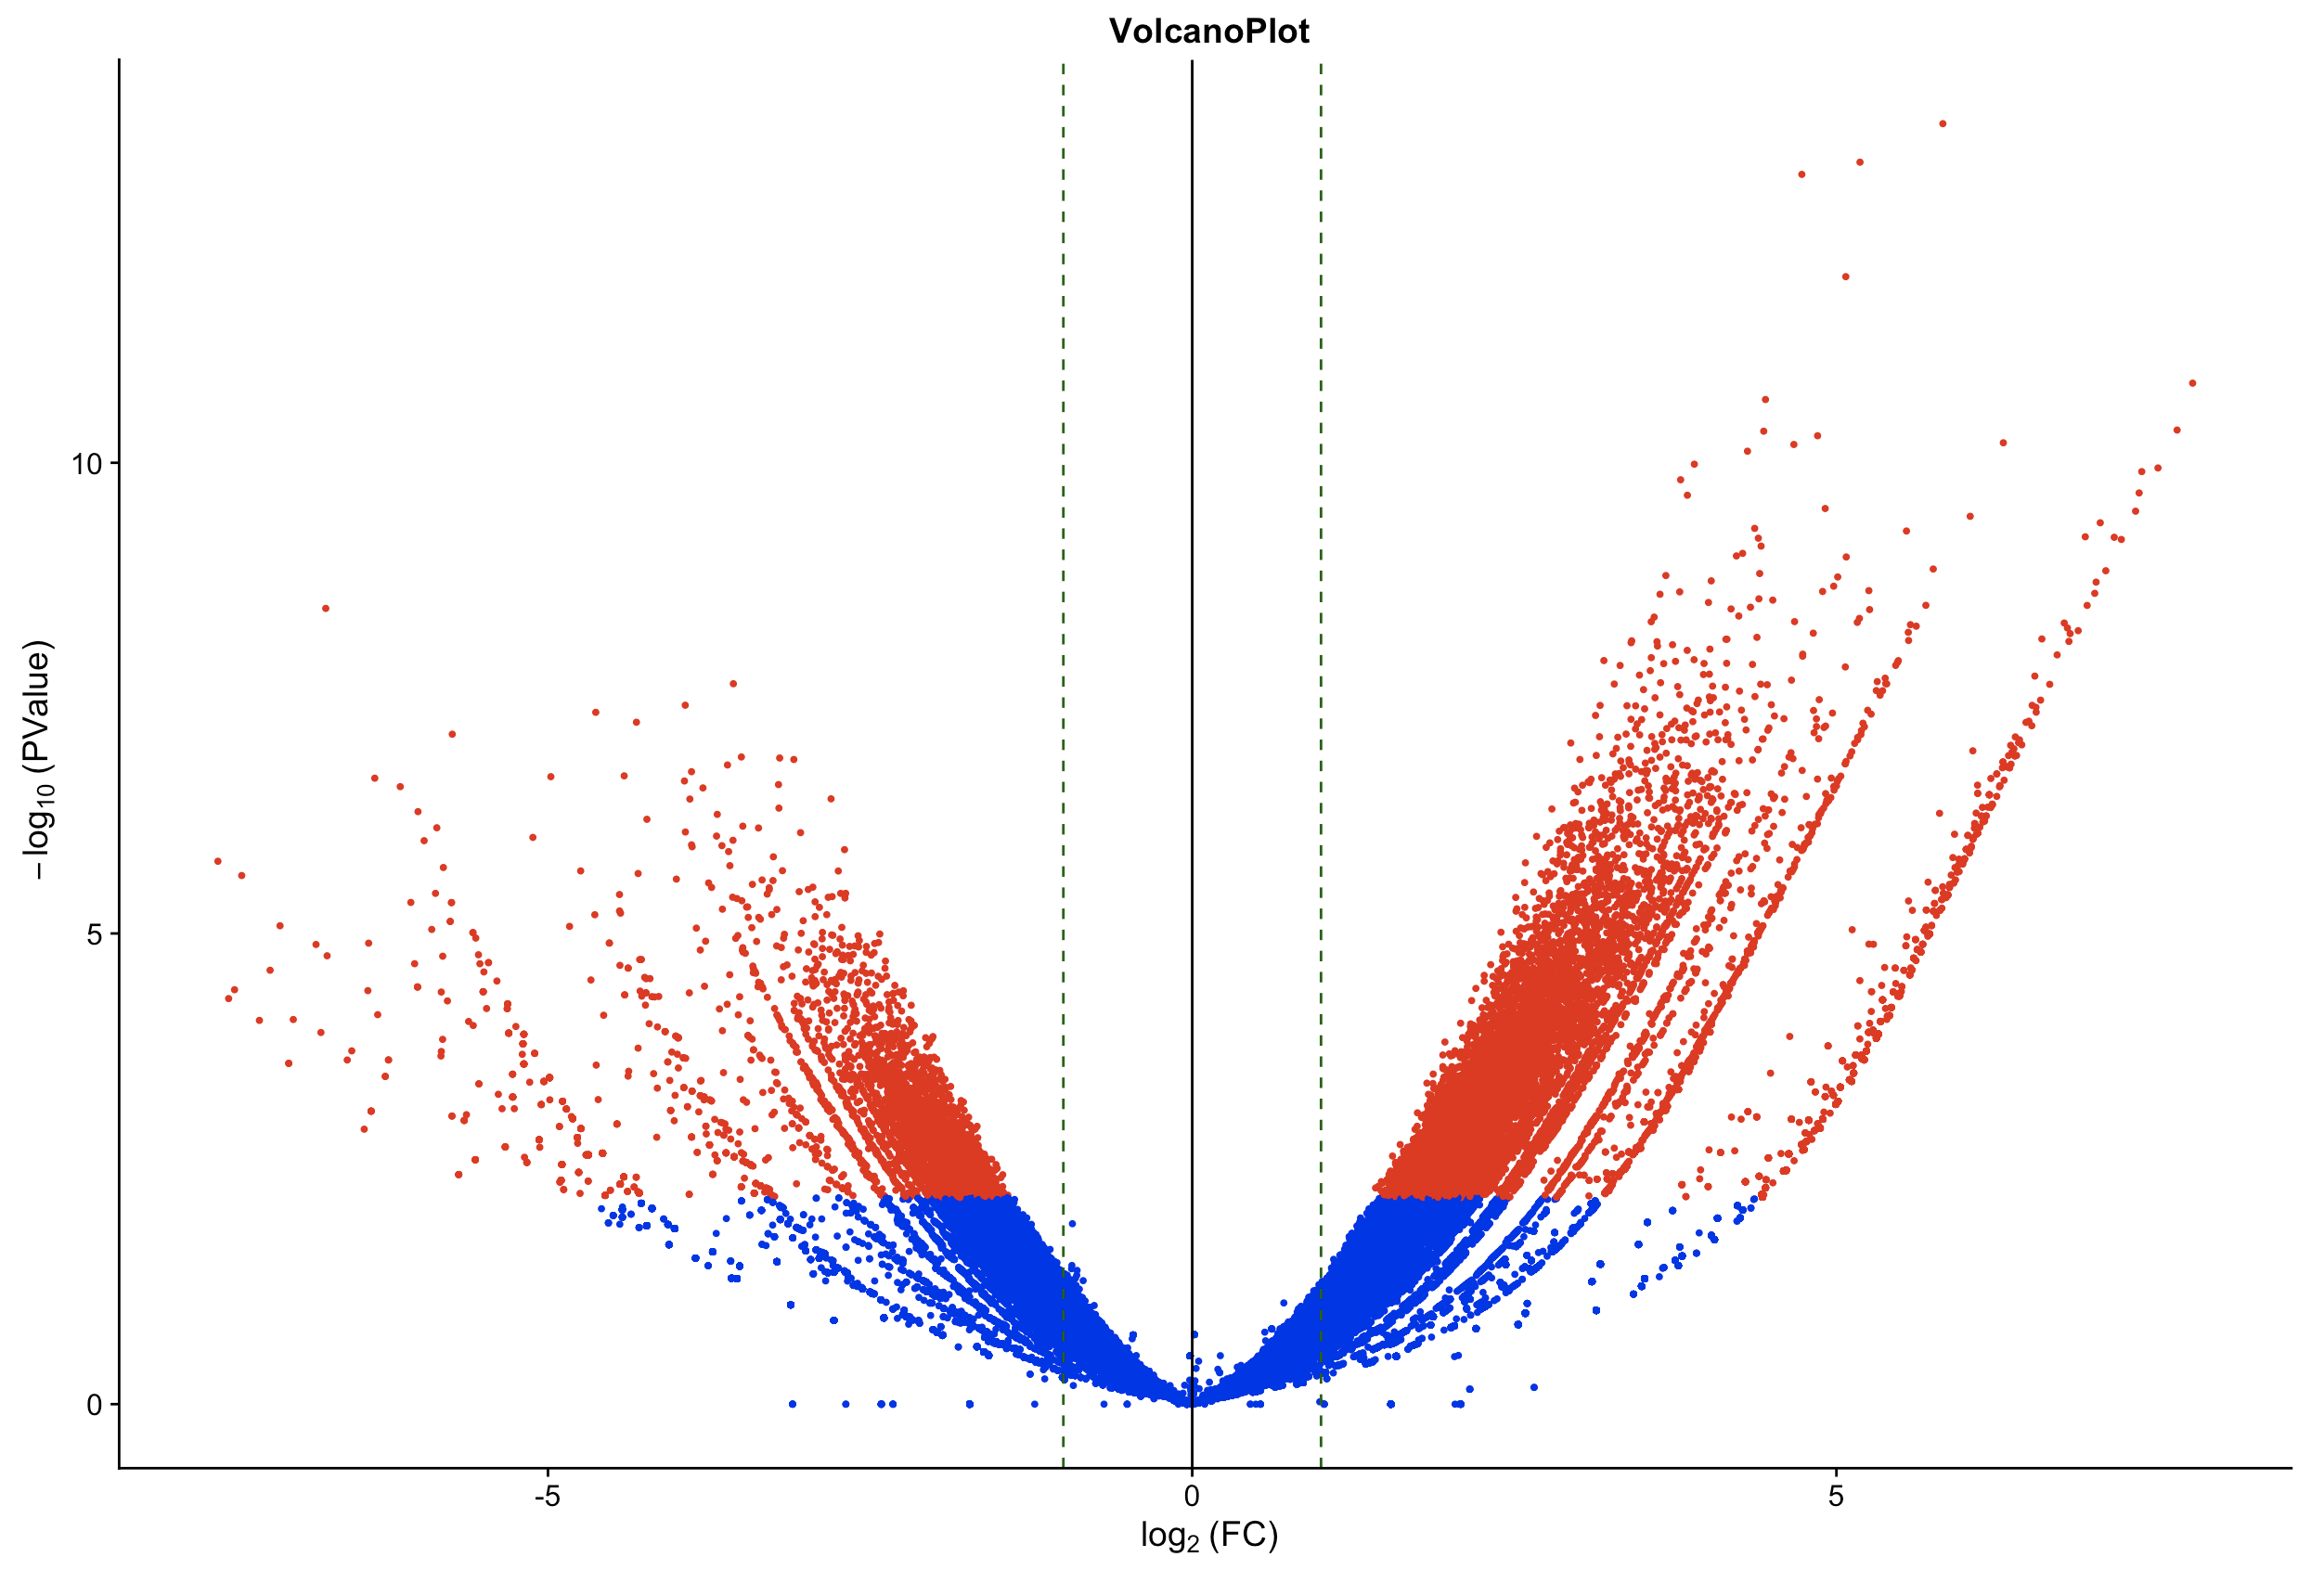
\includegraphics[width=\textwidth, height=\textheight, keepaspectratio]{img/descan2/DE_peaks.png}
\caption[Differential Enrichment Regions Volcano]{A volcano plot of Differential Enriched Regions. Blue dots represent the not significant DERs, while the red ones represent the significant DERs.}
\label{fig:depeaksdescan}
\centering
\end{figure}

